\chapter{Mathematical Background}
\label{MathBack}

In order to understand the mathematical concepts behind the encryption algorithms described here, some basic concepts are explained here. However, you should have a basic knowledge of linear algebra and polynomial calculus.

\section{Lattice}

% Based on \cite{LatticeTutorial}.

All of the algorithms discussed in this thesis are based on lattices, which is why we will briefly focus on them in more detail. In general, lattices behave like any other vector space, but they only consist of discrete vectors. This means that the vectors only contain integers and not real numbers as in a vector space.

Let $B = \{b_1, b_2, \ldots, b_m\}$ be a set of linearly independent vectors of $\mathbb{R}^n$. The lattice $L$ generated by $B$ is the set of integer linear combinations of $B$. $B$ is called the basis of the lattice $L$. That is,
$$L(B) = \{a_1b_1 + \ldots + a_mb_m | a_1, \ldots, a_m \in \mathbb{Z}  \} \subset \mathbb{R}^n$$


Using a matrix $B$, which contains the basis vectors as column vectors, we can generate $L$ equivalently.

$$L(B) = \{Bx | x \in \mathbb{Z}^m  \} \subset \mathbb{R}^n$$

As with this definition, the integer $n$ is the \textbf{dimension} of the lattice and $m$ its \textbf{rank}. If $m = n$ then $L$ is a \textbf{full-rank} lattice, which is the usual case in this Thesis.

An example of an lattice based on an basis $B$ and all points the can be created with that can be seen in Figure \ref{fig:latticeGrid}.

\begin{figure}[h]
    \centering
    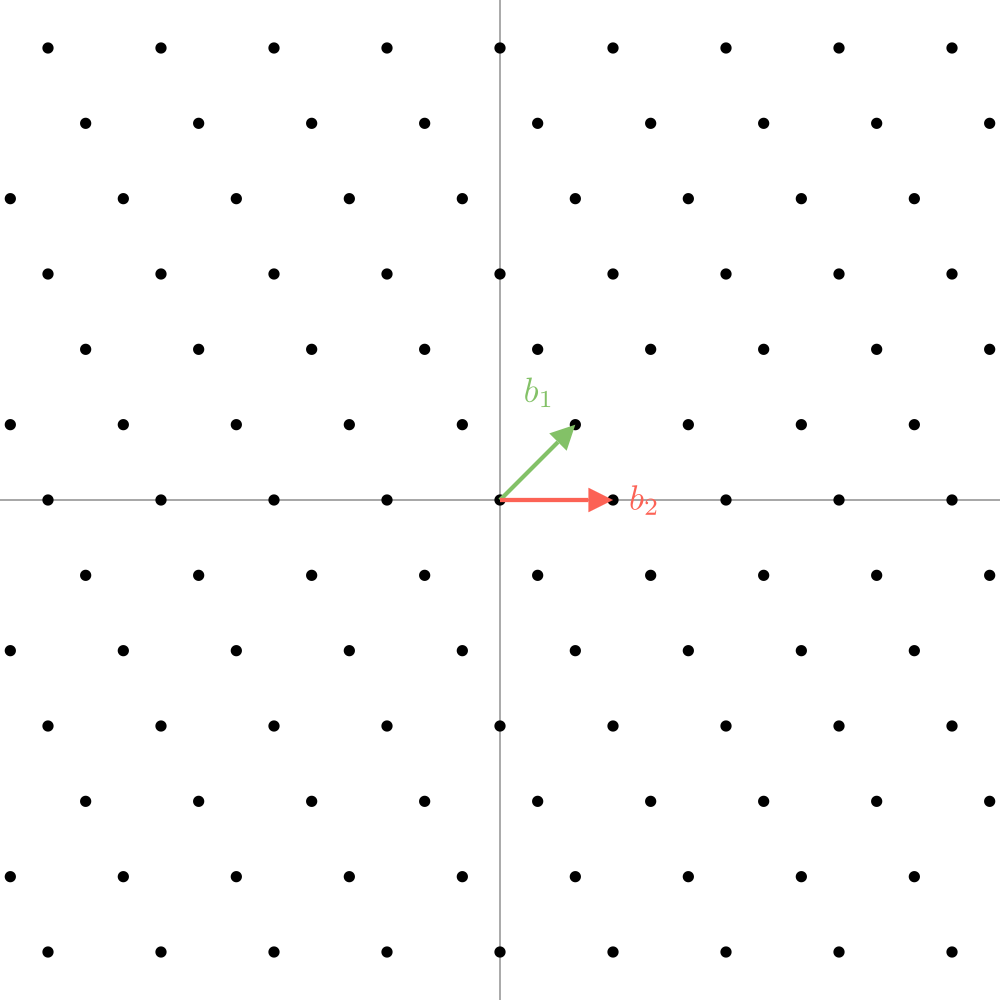
\includegraphics[scale=0.2]{images/LatticeGrid.png}
    \caption[Span of an Lattice]{The span of an two-dimensional lattice with basis  $B = \{b_1, b_2\}$.}
    \label{fig:latticeGrid}
\end{figure}

\section{Shortest Vector \& Closest Vector Problem}

\section{Polynomial Rings}
- explain also the modulus

